% UCL Thesis LaTeX Template
%  (c) Ian Kirker, 2014
% 
% This is a template/skeleton for PhD/MPhil/MRes theses.
%
% It uses a rather split-up file structure because this tends to
%  work well for large, complex documents.
% We suggest using one file per chapter, but you may wish to use more
%  or fewer separate files than that.
% We've also separated out various bits of configuration into their
%  own files, to keep everything neat.
% Note that the \input command just streams in whatever file you give
%  it, while the \include command adds a page break, and does some
%  extra organisation to make compilation faster. Note that you can't
%  use \include inside an \include-d file.
% We suggest using \input for settings and configuration files that
%  you always want to use, and \include for each section of content.
% If you do that, it also means you can use the \includeonly statement
%  to only compile up the section you're currently interested in.
% You might also want to put figures into their own files to be \input.

% For more information on \input and \include, see:
%  http://tex.stackexchange.com/questions/246/when-should-i-use-input-vs-include


% Formatting and binding rules for theses are here: 
%  https://www.ucl.ac.uk/students/exams-and-assessments/research-assessments/format-bind-and-submit-your-thesis-general-guidance

% This package goes first and foremost, because it checks all 
%  your syntax for mistakes and some old-fashioned LaTeX commands.
% Note that normally you should load your documentclass before 
%  packages, because some packages change behaviour based on
%  your document settings.
% Also, for those confused by the RequirePackage here vs usepackage
%  elsewhere, usepackage cannot be used before the documentclass
%  command, while RequirePackage can. That's the only functional
%  difference as far as I'm aware.
\RequirePackage[l2tabu, orthodox]{nag}


% ------ Main document class specification ------
% The draft option here prevents images being inserted,
%  and adds chunky black bars to boxes that are exceeding 
%  the page width (to show that they are).
% The oneside option can optionally be replaced by twoside if
%  you intend to print double-sided. Note that this is
%  *specifically permitted* by the UCL thesis formatting
%  guidelines.
%
% Valid options in terms of type are:
%  phd
%  mres
%  mphil
%\documentclass[12pt,phd,draft,a4paper,oneside]{ucl_thesis}
\documentclass[12pt,phd,a4paper,oneside]{ucl_thesis}


% Package configuration:
%  LaTeX uses "packages" to add extra commands and features.
%  There are quite a few useful ones, so we've put them in a 
%   separate file.

% -------- Packages --------

% This package just gives you a quick way to dump in some sample text.
% You can remove it -- it's just here for the examples.
\usepackage{blindtext}

% This package means empty pages (pages with no text) won't get stuff
%  like chapter names at the top of the page. It's mostly cosmetic.
\usepackage{emptypage}

% The graphicx package adds the \includegraphics command,
%  which is your basic command for adding a picture.
\usepackage{graphicx}

% The float package improves LaTeX's handling of floats,
%  and also adds the option to *force* LaTeX to put the float
%  HERE, with the [H] option to the float environment.
\usepackage{float}

% The amsmath package enhances the various ways of including
%  maths, including adding the align environment for aligned
%  equations.
\usepackage{amsmath}

% Use these two packages together -- they define symbols
%  for e.g. units that you can use in both text and math mode.
\usepackage{gensymb}
\usepackage{textcomp}
% You may also want the units package for making little
%  fractions for unit specifications.
%\usepackage{units}


% The setspace package lets you use 1.5-sized or double line spacing.
\usepackage{setspace}
\setstretch{1.5}


\usepackage{minted}
\usemintedstyle{manni}

\usepackage{listings}





% That just does body text -- if you want to expand *everything*,
%  including footnotes and tables, use this instead:
%\renewcommand{\baselinestretch}{1.5}


% PGFPlots is either a really clunky or really good way to add graphs
%  into your document, depending on your point of view.
% There's waaaaay too much information on using this to cover here,
%  so, you might want to start here:
%   http://pgfplots.sourceforge.net/
%  or here:
%   http://pgfplots.sourceforge.net/pgfplots.pdf
%\usepackage{pgfplots}
%\pgfplotsset{compat=1.3} % <- this fixed axis labels in the version I was using

% PGFPlotsTable can help you make tables a little more easily than
%  usual in LaTeX.
% If you're going to have to paste data in a lot, I'd suggest using it.
%  You might want to start with the manual, here:
%  http://pgfplots.sourceforge.net/pgfplotstable.pdf
%\usepackage{pgfplotstable}

% These settings are also recommended for using with pgfplotstable.
%\pgfplotstableset{
%	% these columns/<colname>/.style={<options>} things define a style
%	% which applies to <colname> only.
%	empty cells with={--}, % replace empty cells with '--'
%	every head row/.style={before row=\toprule,after row=\midrule},
%	every last row/.style={after row=\bottomrule}
%}


% The mhchem package provides chemistry formula typesetting commands
%  e.g. \ce{H2O}
%\usepackage[version=3]{mhchem}

% And the chemfig package gives a weird command for adding Lewis 
%  diagrams, for e.g. organic molecules
%\usepackage{chemfig}

% The linenumbers command from the lineno package adds line numbers
%  alongside your text that can be useful for discussing edits 
%  in drafts.
% Remove or comment out the command for proper versions.
%\usepackage[modulo]{lineno}
% \linenumbers 


% Alternatively, you can use the ifdraft package to let you add
%  commands that will only be used in draft versions
%\usepackage{ifdraft}

% For example, the following adds a watermark if the draft mode is on.
%\ifdraft{
%  \usepackage{draftwatermark}
%  \SetWatermarkText{\shortstack{\textsc{Draft Mode}\\ \strut \\ \strut \\ \strut}}
%  \SetWatermarkScale{0.5}
%  \SetWatermarkAngle{90}
%}


% The multirow package adds the option to make cells span 
%  rows in tables.
\usepackage{multirow}


% Subfig allows you to create figures within figures, to, for example,
%  make a single figure with 4 individually labeled and referenceable
%  sub-figures.
% It's quite fiddly to use, so check the documentation.
%\usepackage{subfig}

% The natbib package allows book-type citations commonly used in
%  longer works, and less commonly in science articles (IME).
% e.g. (Saucer et al., 1993) rather than [1]
% More details are here: http://merkel.zoneo.net/Latex/natbib.php
%\usepackage{natbib}

% The bibentry package (along with the \nobibliography* command)
%  allows putting full reference lines inline.
%  See: 
%   http://tex.stackexchange.com/questions/2905/how-can-i-list-references-from-bibtex-file-in-line-with-commentary
\usepackage{bibentry} 

% The isorot package allows you to put things sideways 
%  (or indeed, at any angle) on a page.
% This can be useful for wide graphs or other figures.
%\usepackage{isorot}

% The caption package adds more options for caption formatting.
% This set-up makes hanging labels, makes the caption text smaller
%  than the body text, and makes the label bold.
% Highly recommended.
\usepackage[format=hang,font=small,labelfont=bf]{caption}

% If you're getting into defining your own commands, you might want
%  to check out the etoolbox package -- it defines a few commands
%  that can make it easier to make commands robust.
\usepackage{etoolbox}

% The microtype package adds `micro-typographic extensions' which
% generally makes text more readable and hyphenation less likely.
\usepackage{microtype}


% Sets up links within your document, for e.g. contents page entries
%  and references, and also PDF metadata.
% You should edit this!
%%
%% This file uses the hyperref package to make your thesis have metadata embedded in the PDF, 
%%  and also adds links to be able to click on references and contents page entries to go to 
%%  the pages.
%%

% Some hacks are necessary to make bibentry and hyperref play nicely.
% See: http://tex.stackexchange.com/questions/65348/clash-between-bibentry-and-hyperref-with-bibstyle-elsart-harv
\usepackage{bibentry}
\makeatletter\let\saved@bibitem\@bibitem\makeatother
\usepackage[pdftex,hidelinks]{hyperref}
\makeatletter\let\@bibitem\saved@bibitem\makeatother
\makeatletter
\AtBeginDocument{
    \hypersetup{
        pdfsubject={Thesis Subject},
        pdfkeywords={Thesis Keywords},
        pdfauthor={Author},
        pdftitle={Title},
    }
}
\makeatother
    


% And then some settings in separate files.
% These settings are partly from:
%  http://mintaka.sdsu.edu/GF/bibliog/latex/floats.html

% They give LaTeX more options on where to put your figures, and may
%  mean that fewer of your figures end up at the tops of pages far
%  away from the thing they're related to.

% Alters some LaTeX defaults for better treatment of figures:
% See p.105 of "TeX Unbound" for suggested values.
% See pp. 199-200 of Lamport's "LaTeX" book for details.

%   General parameters, for ALL pages:
\renewcommand{\topfraction}{0.9}	% max fraction of floats at top
\renewcommand{\bottomfraction}{0.8}	% max fraction of floats at bottom

%   Parameters for TEXT pages (not float pages):
\setcounter{topnumber}{2}
\setcounter{bottomnumber}{2}
\setcounter{totalnumber}{4}     % 2 may work better
\setcounter{dbltopnumber}{2}    % for 2-column pages
\renewcommand{\dbltopfraction}{0.9}	% fit big float above 2-col. text
\renewcommand{\textfraction}{0.2}	% page must be at least 20% text, 
%                                  less than that and we get a floatpage

%   Parameters for FLOAT pages (not text pages):
\renewcommand{\floatpagefraction}{0.7}	% require fuller float pages
% N.B.: floatpagefraction MUST be less than topfraction !!
\renewcommand{\dblfloatpagefraction}{0.7}	% require fuller float pages

% remember to use [htp] or [htpb] for placement,
% e.g. 
%  \begin{figure}[htp]
%   ...
%  \end{figure}
 % For things like figures and tables
\bibliographystyle{unsrt}

   % For bibliographies

% These control how many number sections your subsections will take
%    e.g. Section 2.3.1.5.6.3
%  and how many of those will get put into the contents pages.
\setcounter{secnumdepth}{3}
\setcounter{tocdepth}{3}


\begin{document}

\hypersetup{
     colorlinks=true,
     linkcolor=blue,
     filecolor=blue,
     citecolor = blue,      
     urlcolor=cyan,
     }



% ^-- This is a dumb trick that works with the bibentry package to let
%  you put bibliography entries whereever you like.
% I used this to put references to papers a chapter's work was 
%  published in at the end of that chapter.
% For more information, see: http://stefaanlippens.net/bibentry

% If you haven't finished making your full BibTex file yet, you
%  might find this useful -- it'll just replace all your
%  citations with little superscript notes.
% Uncomment to use.
%\renewcommand{\cite}[1]{\emph{\textsuperscript{[#1]}}}

% At last, content! Remember filenames are case-sensitive and 
%  *must not* include spaces.
% I may change the way this is done in a future version, 
%  but given that some people needed it, if you need a different degree title 
%  (e.g. Master of Science, Master in Science, Master of Arts, etc)
%  uncomment the following 3 lines and set as appropriate (this *has* to be before \maketitle)
% \makeatletter
% \renewcommand {\@degree@string} {Master of Things}
% \makeatother

\title{A Thesis Title}
\author{Author Name}
\department{Department of Something}

\maketitle
\makedeclaration

\begin{abstract} % 300 word limit
My research is about stuff.

It begins with a study of some stuff, and then some other stuff and things.

There is a 300-word limit on your abstract.
\end{abstract}

\begin{impactstatement}

	UCL theses now have to include an impact statement. \textit{(I think for REF reasons?)} The following text is the description from the guide linked from the formatting and submission website of what that involves. (Link to the guide: {\scriptsize \url{http://www.grad.ucl.ac.uk/essinfo/docs/Impact-Statement-Guidance-Notes-for-Research-Students-and-Supervisors.pdf}})

\begin{quote}
The statement should describe, in no more than 500 words, how the expertise, knowledge, analysis,
discovery or insight presented in your thesis could be put to a beneficial use. Consider benefits both
inside and outside academia and the ways in which these benefits could be brought about.

The benefits inside academia could be to the discipline and future scholarship, research methods or
methodology, the curriculum; they might be within your research area and potentially within other
research areas.

The benefits outside academia could occur to commercial activity, social enterprise, professional
practice, clinical use, public health, public policy design, public service delivery, laws, public
discourse, culture, the quality of the environment or quality of life.

The impact could occur locally, regionally, nationally or internationally, to individuals, communities or
organisations and could be immediate or occur incrementally, in the context of a broader field of
research, over many years, decades or longer.

Impact could be brought about through disseminating outputs (either in scholarly journals or
elsewhere such as specialist or mainstream media), education, public engagement, translational
research, commercial and social enterprise activity, engaging with public policy makers and public
service delivery practitioners, influencing ministers, collaborating with academics and non-academics
etc.

Further information including a searchable list of hundreds of examples of UCL impact outside of
academia please see \url{https://www.ucl.ac.uk/impact/}. For thousands more examples, please see
\url{http://results.ref.ac.uk/Results/SelectUoa}.
\end{quote}
\end{impactstatement}

\begin{acknowledgements}
Acknowledge all the things!
\end{acknowledgements}

\setcounter{tocdepth}{2} 
% Setting this higher means you get contents entries for
%  more minor section headers.

\tableofcontents
\listoffigures
\listoftables


\chapter{Introduction}
\label{chapterlabel1}

Good software development does not just entail writing functional code. Factors that don't impact the final output of the code, like clear well written syntax, inclusion of code testing, and making efficient use of CPU resources for the task at hand can significantly increase the usability and reliableness of software in a research setting. This thesis focuses on making efficient use of CPU resources, or more intuitively writing code that does the required task as fast as is possible with the tools at hand. The project focuses in particular on the \textbf{Contur} package, which is an open source software used in particle physics to test the consistency of theoretical predictions from newly proposed physics models against realised experimental data. The project entailed profiling the \textbf{Contur}  code base and from the profile results identifying parts of the code where potential inefficiencies exist which can be improved upon. A brief summary of the contents of each chapter of this thesis follows below.

To start the thesis in Chapter 2 we attempt to provide the necessary \textbf{Contur} background. This background contains a brief sketch of the current situation within particle physics research that creates a gap for a tool like \textbf{Contur} to be useful, followed by an overview of the \textbf{Contur}  package itself in terms of what it does and how it works. The outline of the workings of \textbf{Contur}  will be necessarily brief but should be sufficient to give the reader the required background to understand later changes made to better optimise the code.

From Chapter 3 on in this thesis we start to discuss work actually carried out by this author as part of the research project. Chapter 3 specifically begins with a discussion of the benefits to \textbf{Contur} users arising from the improved runtime which will result from code efficiencies. The chapter then moves onto outlining the tools used to perform and visualise the profiling results. The chapter then concludes by presenting the profiling results for the last version of \textbf{Contur} that exists before we started this project. This initial profile is taken as the benchmark to judge the effectiveness of later attempts to optimise \textbf{Contur}.

In Chapter 4 we digress slightly from the main theme of the project to discuss introducing automatic tests into the \textbf{Contur} package. When making code changes in \textbf{Contur} for optimisation purposes, an important consideration is that we don't unintentional break or introduce errors into the code. Especially errors that will have an impact on the final output of the code. One means we can reduce the chances of introducing errors is via robust testing infrastructure. Chapter 4 outlines the step taken as part of this research project to improve \textbf{Contur's} testing infrastructure.

Chapter 5 then finally outlines the changes made to \textbf{Contur}  as part of this research project. Each of the changes outlined has been made because they can carry out the exact same process as the existing \textbf{Contur}  code in a more efficient way. For each change made we give the background necessary to understand the purpose of the section of code we are changing, we explain the change we made and we give updated profiling results showing the impact of the change in terms of run time.

We will then conclude the thesis in Chapter 6 by summarising the accomplishments of the project. Additionally the final profile results of \textbf{Contur}  after all the optimisation changes have been implemented will be presented. From these final results we can understand the most computational intensive remaining parts of a \textbf{Contur}  run thus providing the target areas for future optimisation attempts with \textbf{Contur}.  


\chapter{Contur Overview}
\label{chapterlabel2}

\section{Contur and the Standard Model}
The standard model (SM) of particle physics is the name for the collective of quantum field theories that successfully describe three of the four fundamental forces of nature\footnote{The forces successfully described are the electromagnetic force, the weak force and the strong force, while a quantum theory of gravity still eludes us} and the observable matter content of the universe. The success of the SM is evidenced by the generally strong agreement between SM predictions and experimental data. Despite this success there is a widespread view that the SM is not the complete picture. This viewpoint arises from the inability of the SM to accommodate gravity or provide any insight into postulated quantities like dark matter\footnote{Dark matter is hypothetical form of matter postulated to explain discrepancies between observed astrophysical motion and what we would expect based off the gravitational equation of motion in general relativity} and dark energy\footnote{Dark energy is a hypothetical force postulated to explain the observed expansion of the universe}. As a result the task of the developing new fundamental theories in physics that extend the SM, which we will term Beyond Standard Model theories, is an active area of research.

\textbf{Contur}(Constraints On New Theories Using Rivet) has been developed to aid the search for new BSM theories. The approach aims to leverage the large amount of experimental data produced at the Large Hadron Collider to set constraints on the type of BSM theories which are possible. This is done by considering experimental results which have already been shown to agree with SM expectations. The \textbf{Contur} procedure then asks  the question for a given completely specified BSM theory, where by completely specified we mean that the values of all free parameters have been set, \say{at what significance do existing measurements which agree with the SM already exclude this BSM}. 

The approach thus checks the consistency of predictions of the BSM theory against experimental results that have already been shown to align well with SM predictions. The idea being if the BSM theory is inconsistent with the experimental data and fails to predict processes accurately that are already well understood within the SM, then the BSM with parameter values we specified is not viable. Through running \textbf{Contur} for the BSM theory for multiple different free parameter values we can rule out parameter values which are inconsistent with realised data or potentially even rule out the whole BSM theory if there are no values for the free parameters of the BSM theory that produce consistent predictions.

\section{Input Data}\label{data}

\textbf{Contur's} consistency checks compare simulated data from a new BSM theory against realised experimental data. We will now outline in greater detail how these two main sources of data are sourced.

\subsection{Simulated BSM Data}

At first sight the need to produce a large amount of simulated results for a BSM theory for a \textbf{Contur} run would seemingly jeopardise the desire that \textbf{Contur} to be a relatively quick and easy way to check the consistency of the BSM theory with realised data. If for every BSM theory run on \textbf{Contur} scripts of bespoke ancillary code was necessary to produce simulations of the BSM theory something like the \textbf{Contur} procedure would likely not be practicable. 

Fortunately there exists mature packages in the particle physics community specifically devoted to the tasks of simulating particle collision events. These packages are sufficiently flexible that they can be used to simulate both SM events and a wide array of BSM events. A large part of this flexibility comes from the Universal FeynRules Output (UFO)\cite{ufo}, which allows the encoding of the Feymann diagram information of a process in a standard form which can then be passed to an event generator which can use Monte Carlo methods to simulate the event in question.

\textbf{Contur} is event generator agnostic in the sense that any generator that can produce simulations with data in the required final format could be used. Yet, despite this, the main event generator currently used by \textbf{Contur} is \textbf{Herwig}\cite{herwig} and the default assumption within the current set up is that the user generates BSM data with \textbf{Herwig}. For a fully specified BSM theory \textbf{Herwig} will generate events for a range of scenarios, with the output of these simulations being a collection of histograms\footnote{See figure \ref{fig:example_histogram} below for an example of a histogram used}, where any given bucket in these plots is the number of signal events which were counted in that bucket for the BSM theory. All of this output is stored in a single \textbf{YODA} file\cite{yoda}, this \textbf{YODA} file contains all the simulation data required to run \textbf{Contur} for a fully specified BSM theory.

\begin{figure}[H]
\centering
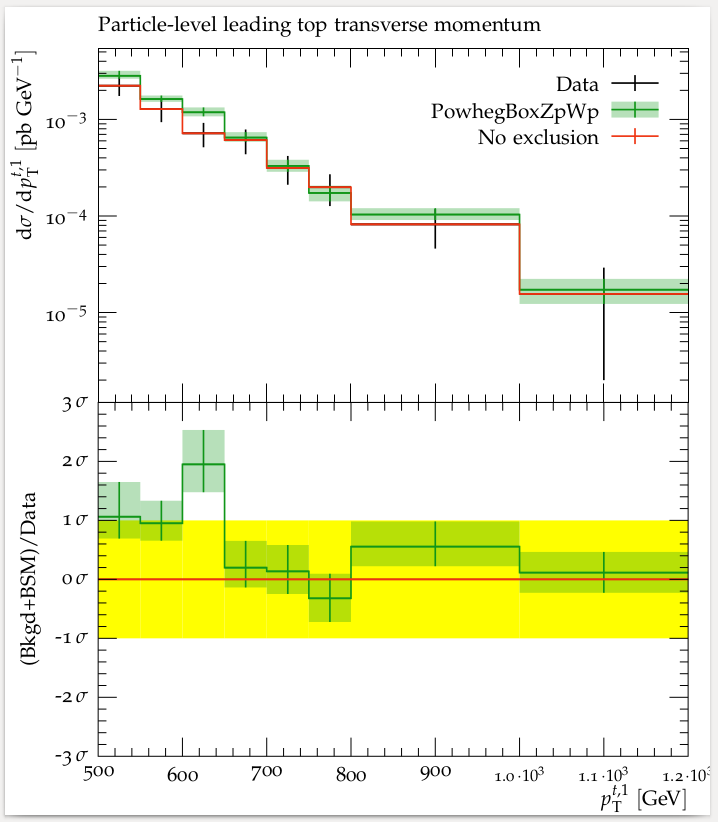
\includegraphics[scale=0.3]{plots/example_histogram.png}
\caption{Example of histogram used in Contur}
\label{fig:example_histogram}
\end{figure}

Recall that we previously defined a fully specified BSM theory to be the BSM with all free parameters given a single value. So running \textbf{Contur} on one fully specified BSM will only check the consistency of the BSM for the parameter values we have specified, different parameter values for the BSM will possible give different signal events changing the output. Thus for any given BSM it is likely to be the case that we want to produce multiple \textbf{YODA} files containing simulated signal events for the BSM using different parameter values across \textbf{YODA} files. 

\textbf{Contur} has tools to create a collection of such \textbf{YODA} files which is termed a grid. These tools sit within \textbf{Contur's} batch process capabilities\footnote{See Chapter 4 of the \textbf{Contur} User Manuel\cite{contur_manuel} for further details}. It is easiest to understand this process if we think of a simple example if we have a BSM theory with just two free parameters with values that can range from $1$ to $10$\footnote{For simplicity take the parameters to be dimensionless}, from this \textbf{Contur} batch can create a grid a $10\times 10$ grid of $100$ \textbf{YODA} files\footnote{\textbf{YODA} file one will be when both parameters have values 1, \textbf{YODA} file two the first parameter will have value 1, the second value 2 etc....}. We can then pass this grid to \textbf{Contur} and run a consistency check for each point on the grid, this is an example of a \textbf{Contur} grid run. The grid run is the main area of \textbf{Contur} we will later focus on in our optimisation efforts.

\subsection{Experimental Data}

Contur sources experimental data via a combination of the HepData\cite{HEPData} repository and Rivet\cite{Rivet}. The HepData repository contains a digitized record of detector level results for run experiments. The Rivet library contains a collection of routines to account for the specifics of the detector and convert the detector level results to particle level result independent of detector effects. These particle level measurements can then be directly compared with the particle level signal effects simulated by the BSM. Carrying out the comparison at particle level ensures that the results being compared do not contain theory dependent extrapolations within them, making the Contur constraints arrived independent of theoretical assumptions. 

The interface with Rivet is built into Contur, so the user does not need to provide any Rivet input when initiating a Contur run. Instead from experiments simulated in the BSM data passed in the yoda file Contur can call pull the appropriate experimental data from Rivet and HepData. In addition to realised results for experiments, simulated SM expectations can also be sourced from Rivet. These simulated SM expectations are created in the same way as the BSM simulations discussed in the previous subsection and stored in yoda files that can be accessed via Rivet. In its default run Contur does not make use of SM expectations, however there exists on optional theory run in Contur which we will discuss in the next section which makes use of SM expectations.


\section{Calculating Likelihoods}\label{calculate_likelihood}

The final output of a \textbf{Contur} run on a single \textbf{YODA} file is a single $CL_s$ exclusion limit, given in the form of the CL(s) technique\cite{cls}. This exclusion limit is an expression of our confidence that a fully specified BSM theory produces signal events inconsistent with understood SM processes.  The calculation of these exclusion limits is the core of the \textbf{Contur} procedure, we will now give a high level overview of the steps involved in this calculation, let us start with the default \textbf{Contur} run on a single \textbf{YODA} file.

The $CL_s$ exclusion limit is defined to be a ratio of p-values,
$$ CL_s: = \frac{CL_{s+b}}{CL_{b}} = \frac{p_{s_b}}{1- p_{b}}, $$
where in the above $p_{s+b}$ is defined as the p-value for the signal plus the background event and $p_{b}$ is the p-value just for the background event. For each histogram \textbf{Contur} computes one $CL_{s}$ by either taking the maximum $CL_{s}$ out of all the bins that compose the histogram or if correlation information between the bins exists using this to compute a single $CL_s$ for the histogram. For any given bin in a histogram, for the default \textbf{Contur} run $p_b$ will always be a half, because we are just comparing the background data with itself, so $p_{s+b}$ will compute the quantity of interest, namely how well the signal count for the BSM approach aligns with the realised count. The below code snippet shows a simplified example of the  flow of the code for the $CL_s$ calculation, the calculation takes place within the \classname{likelihood} class within \textbf{Contur}.

\begin{code}
\captionof{listing}{Compute CLs For Histogram}
\label{code:histo}
\begin{minted}{python}

def EvaluateHistogram(Histogram):
    if Histogram has correlation and (build correlation =True)
          return Likelihood(Histogram)
    else:
          return max(Likelihood(Histogram.bins))
\end{minted}
\end{code}

After computing a $CL_{s}$ for each histogram the next step is to bucket the histograms into statistically independent pools. In \textbf{Contur} a pool is combination of the final particle state, the experiment and the beam energy of the experiment, each of the three chosen so that their combination is statistical independent. Histograms that share these three properties are grouped into the same pool. \textbf{Contur} then takes the histogram with the maximum $CL_s$ in each pool. A snippet of example code to used to carry out this process for a single pool is given below

\begin{code}
\captionof{listing}{Sort Likelihood blocks into pools}
\label{code:pools}
\begin{minted}{python}

def EvaluatePool(Pool):
    scores = [] #empty list for results
    if Histogram in pool:
       scores.append(EvaluateHistogram(Histogram))
    return Histogram with max(scores)
\end{minted}
\end{code}

Finally \textbf{Contur} takes the histograms from each pool and combines into a single histogram to calculate a final $CL_s$ for the \textbf{YODA} file. In combining histograms like this \textbf{Contur} assumes each of the pools to be statistical independent, which they are by construction. A simplified example of the code to perform this step is given by

\begin{code}
\captionof{listing}{Build Full Likelihood}
\label{code:full_likelihood}
\begin{minted}{python}

def BuildFullLikelihood():
      tests = []
      for Pool in ConturPools:
            tests.append(EvaliatePool(Pool))
       return Likelihood(tests)
\end{minted}
\end{code}

The main alternative run option also available in \textbf{Contur} is a theory run. In the theory run when computing the background p-value $p_b$, instead of just trivially comparing the data with itself, the SM expectations are used. So the theory \textbf{Contur} run provides more of a relative measure of which of the SM expectations or BSM expectations are in better agreement with the realised data.

As already highlighted the most common way \textbf{Contur} is used in practice is on a grid of \textbf{YODA} files as opposed to just a single file. The \textbf{Contur} grid run is not fundamentally different from the single \textbf{YODA} run, for the grid run \textbf{Contur} runs iteratively through all the \textbf{YODA} files in the grid, at each iteration calculating a single final $CL_{s}$ for the \textbf{YODA} file at that point. So the final output of the \textbf{Contur} grid run is a $CL_{s}$ value for each point on the grid. This grid of $CL_{s}$ values output can be presented as a heat map, an example of which can be seen in figure 


\begin{figure}[H]
\centering
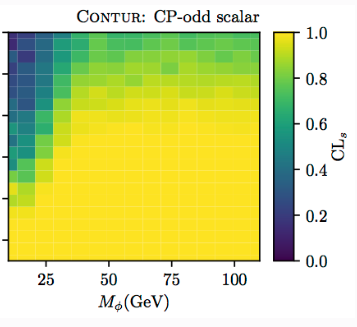
\includegraphics[scale=1]{plots/example_heatmap.png}
\caption{Example of heat map from grid run}
\label{fig:example_heatmap}
\end{figure}

\chapter{Profiling Contur}
\label{chapterlabel3}

Before any attempt can be made to optimise code within \textbf{Contur}, it is first necessary to identify processes within the code where potential inefficiencies exist and we can make improvements. The best way to do this is to perform a profile of the code. A good profile should give us visibility not just on the total runtime of \textbf{Contur}, but how this runtime breaks down between the different processes that compose a \textbf{Contur} run. 

This section will outline the steps taken to produce a profile of \textbf{Contur} and how we used the results. We will start by introducing \textbf{cProfile}, which is the Python profiler which was used to carry out the profile. Then we will discuss \textbf{Snakeviz} and \textbf{gprof2dot}, these are the two tools which we used to visualise the profiling results produced by \textbf{cProfile}. Finally we will conclude the section by performing an initial profile of the \textbf{Contur} package before any code optimisation was attempted. This initial profile will serve as our benchmark to measure the effectiveness of our later attempts to improve the run time performance of \textbf{Contur}.

First however let us briefly consider why it is a worthwhile effort to try and improve the runtime of \textbf{Contur} code.

\section{Why attempt to optimise Contur?}
The obvious answer to the question \say{Why attempt to optimise \textbf{Contur}?} is simple that we will have code that runs faster. The immediate benefit of faster code for a researcher using \textbf{Contur} is that the wait time from run initiation to results is reduced, all else equal this should increase productivity.

We can argue further though that faster code increases the range of analysis that a researcher can perform with \textbf{Contur}. This argument follows from the observation that there likely exists a runtime above which \textbf{Contur} becomes impractical to use as a research tool\footnote{To take an extreme example, if the code takes over 24 hours to run, its utility to a researcher will be much less than code that takes under an hour to run.}. If we combine with this the observation that will be discussed later in Chapter \ref{chapterlabel5} that the runtime increases with the size of the grid used, then we can see that runtime puts an upper bound on the size of the grid that can be run with \textbf{Contur}. Improving run time will thus likely increase this upper bound which would allow researchers either to increase the span of a parameter space they evaluate, or look a the parameter space with a greater level of granularity.

A final obvious benefit of runtime improvements follows from the fact that currently grids that are too large to run locally will be run on a HPC cluster. Increasing the range of grids that can be run locally will thus decrease the volume of runs going to the cluster, saving valuable CPU resources. Additionally for grids that still need to go to the cluster, making \textbf{Contur} code more efficient will reduce wasteful usage of the HPC CPU resources.

\section{Profiling with cProfile}

\subsection{Why cProfile?}
Let us consider some of the features we ideally require from our chosen profiler. At a minimum a profiler must obviously be able to time how long it takes our code to run. This basic requirement is essential to be able to determine if our attempted improvements to the code do in fact actually improve run performance. In addition to just providing the total runtime of \textbf{Contur} we will also require our profiler to provide a split of the runtime among the functions/sub-functions which compose \textbf{Contur}. A split of the runtime like this will highlight parts of the code that consume disproportionately large amounts of CPU or are repetitively called, suggesting optimisation improvements can be made.

\textbf{cProfile}\cite{cProfile} is a module within the Python standard library which meets these requirements. Our main motivations for using \textbf{cProfile} are as follows:

\begin{itemize}
\item Provides a full profile of program with output include total run time, time taken at each individual step, and number of calls to individual functions;
\item Easy to save the output of the profile in \texttt{prof} files which can then be read by tools built to visualise profiling results;
\item Performing the profile with \textbf{cProfile} is quick and easy and requires minimal new code;
\end{itemize}

\subsection{Using cProfile}
We will demonstrate the usage of \textbf{cProfile} by profiling the last version of \textbf{Contur} which existed before any optimisation attempts were made\footnote{The version can be found in commit \href{https://gitlab.com/hepcedar/contur/-/tree/49a67e039cf93c88b39dade3dfb7c5f03e780fb2}{49a67e03}}. All \textbf{Contur} code can be found in the main \textbf{Contur} repository\cite{contur_main}, additionally all code contributions for this thesis can also be found as a commits in the main repository\footnote{See appendix \ref{appendixlabel2} for more details}. 

For the demonstration we will walk through the steps to profile a single \textbf{YODA} file. The steps required to perform the profile on a \textbf{Contur} grid run are the same, so at the conclusion of this chapter we can just provide the profiling results for the grid run without repeating the walk through.

The simplest way of performing a profile with \textbf{cProfile} is via \textbf{cProfile's} \texttt{run} method. To profile \textbf{Contur} using the run method we just pass \textbf{Contur's} main function to the \texttt{run} method. We make this adjustment to \textbf{Contur's} code by updating the main run script\footnote{Can be found \href{https://gitlab.com/hepcedar/contur/-/blob/main/bin/contur}{here}} in listing \ref{code:first_profile} below.

\begin{code}
\captionof{listing}{Example using \textbf{cProfile} run}
\label{code:first_profile}
\begin{minted}{python}
import cProfile

if __name__ == "__main__":
       cls_args = get_args(sys.argv[1:],'analysis')
       cProfile.run("main(cl_args)", sort=cumtime)
\end{minted}
\end{code}


After updating the run script as above we can now run \textbf{Contur} as normal to get the below terminal output from the profile

\begin{figure}[H]
\centering
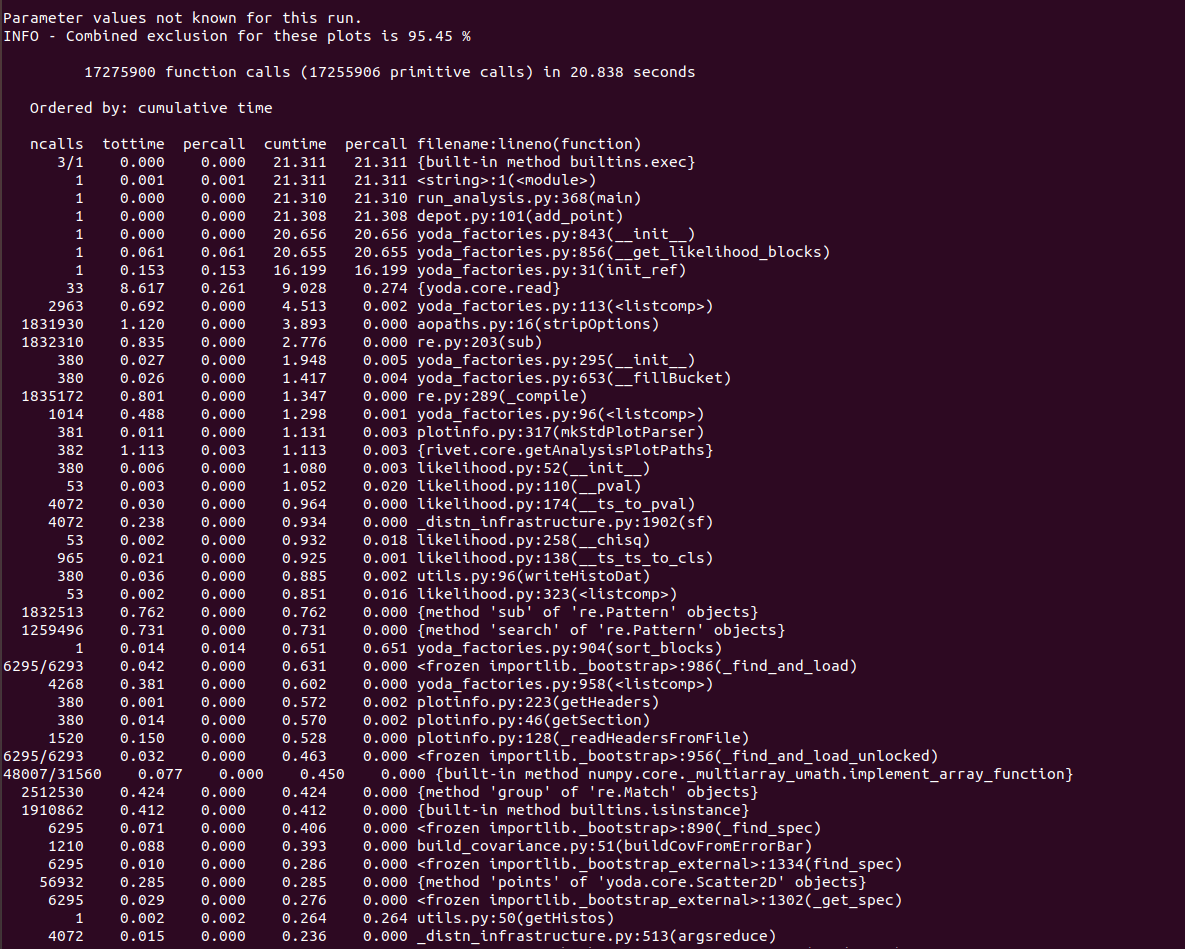
\includegraphics[scale=0.35]{plots/example_profile.png}
\caption{Output of \textbf{cProfile} run method}
\label{fig:ep}
\end{figure}

From figure \ref{fig:ep} above we can summarise the main output from the single \textbf{YODA} file \textbf{Contur} run:

\begin{itemize}
\item From line one of the profiling results we can see that the run had c.a. 17 million function calls and took c.a. 20 seconds to run;
\item The next line tells us that we are ordering the profiling results by cumulative time (\texttt{cumtime} column). The cumulative time for a function is the time spent to run a function and all other functions called within the function (so the \texttt{cumtime} for the main function will be the total run time of the program as all other functions are called within main);
\item From line three on we have the profiling information for the functions and sub-functions which compose the \textbf{Contur}  run. The main columns which stand out here are \texttt{ncalls} which gives the number of calls made to the function, \texttt{tottime} which gives the total time spent in the function excluding calls to sub functions and finally \texttt{cumtime} which as already explained gives the run time for each function including all the calls to sub functions;
\end{itemize}

The above profiling is already useful, it gives us things like the run time and the break down of the run time between the components of \textbf{Contur} . However the printed results in the current form are not very readable, a detailed knowledge of the functions that compose \textbf{Contur} would be needed to take any advantage of the run time broken down by components in its current form. Additionally we don't just want to print result to the terminal and work from there, we would preferable save the profiling results to some file format so our results are reusable across time. 

To meet both these objectives for the profiling we  from here on we will print the data from our profile into \texttt{prof} files which can then be read by tools which help visualise the profiling results. We do this by introducing the Profile class of \textbf{cProfile} and using this to perform our profiles from here on in as opposed to using the run method, the updated code to perform the profiling with the \textbf{cProfile} class is given in listing \ref{code:second_profile} below.

\begin{code}
\captionof{listing}{Modification to \textbf{Contur} run for \textbf{cProfile}}
\label{code:second_profile}
\begin{minted}{python}
import cProfile, pstats, io

if __name__ == "__main__":
       cls_args = get_args(sys.argv[1:],'analysis')
       
       pr = cProfile.Profile()
       pr.enable()
       
       main(cl_args)
       
       pr.disable()
       pr.dump_stats('outfile.prof'')
\end{minted}
\end{code}


\section{Visualizing Profiling Results}

To visualise our profiling results we will use two open source tools \textbf{Snakeviz} and \textbf{gprof2dot}. As what follows will show, we can use both of these tools in a complementary way, as opposed to a simple choose of one or the other, to help make best of use of the profiling data we produce with \textbf{cProfile}.

\subsection{Snakeviz}\label{snakeviz}
\textbf{Snakeviz}\cite{snakeviz} is a browser based graphical viewer for the output of Python's \textbf{cProfile} profiler module. \textbf{Snakeviz} can easily be pip installed with the following terminal command

\begin{minted}{bash}
  $ pip install snakeviz
\end{minted}

once installed we can invoke \textbf{Snakeviz} to visualise an arbitrary \texttt{prof} file as follows

\begin{minted}{bash}
  $ snakeviz profile_file.prof
\end{minted}

After invoking \textbf{Snakeviz} as outlined above the web browser interface for the tool will open and the user can explore the profiling results. \textbf{Snakeviz} allows user interaction to adjust how results are rendered, the two main plotting options available in \textbf{Snakeviz} are icicle plots and sunburst plots\footnote{A nice overview of these plots in \textbf{Snakeviz} can be found \href{https://www.machinelearningplus.com/python/cprofile-how-to-profile-your-python-code/}{here}}. 

From here on we will use \textbf{Snakeviz's} icicle plot to explore profiling results, additionally due to the constraints of the static form of this document is written in we will just examine static snapshots of the overall display in \textbf{Snakeviz's} viewer. These static snapshots of the \textbf{Snakeviz} viewer are sufficient to summarise profiling results. Using \textbf{Snakeviz's} viewers ability to adjust rendering though can be useful to get a feel and understanding for new profiling results, the interested reader is recommended to play around with \textbf{Snakeviz's} viewer functionality further\footnote{See appendix \ref{appendixlabel1} for information on where to find \texttt{prof} files associated with work carried out for this project }.

Below in figure \ref{fig:single_yoda_start_profile_snakeviz} we show a snapshot of an icicle plot from a profile of our initial starting \textbf{Contur} code on a single \textbf{YODA} file. From the figure we can seen that the icicle plot is showing the same information as figure \ref{fig:ep} in just a more visually appealing way, with the addition that in the icicle plot we can see the ordering of the calls to the components of code that compose a \textbf{Contur} run. This ordering is very useful additional information, for example from the ordering it jumps out at us that the call to \texttt{yoda.core} to read the \textbf{YODA} file passed to \textbf{Contur} takes a large proportion of the run time for a single \textbf{YODA} run. From this we can already understand that a lot of the run time for a single \textbf{YODA} run comes from just reading in data. 

\begin{figure}[H]
\centering
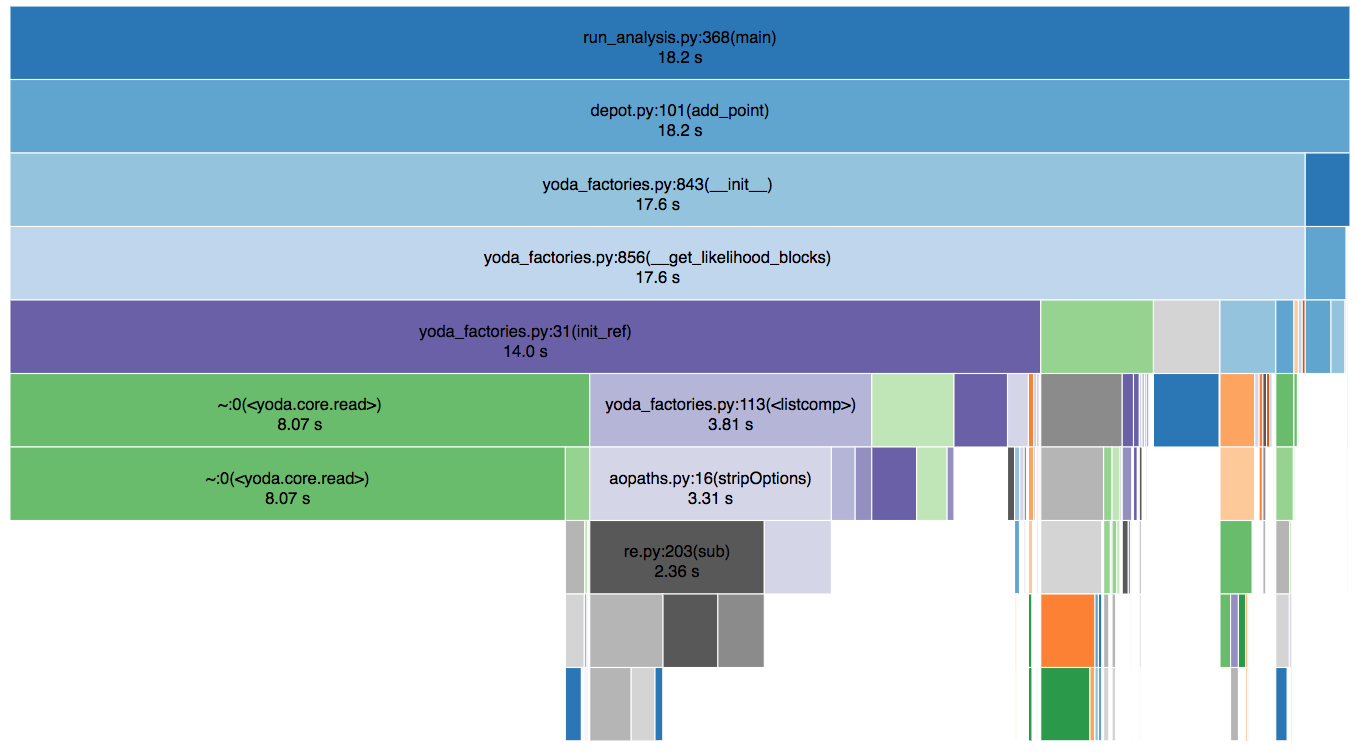
\includegraphics[scale=0.3]{plots/initial_single_contur.png}
\caption{\textbf{Contur} single \textbf{YODA} run starting point - Example \textbf{Snakeviz} icicle plot}
\label{fig:single_yoda_start_profile_snakeviz}
\end{figure}

\subsection{gprof2dot}\label{dot_plot}
\textbf{gprof2dot}\cite{gprof2dot} is a python script that converts the output of the \textbf{cProfile} to dot plots. These dot plots can be used to complement the information we get from the icicle plots. The icicle plots and the user interface offered by \textbf{Snakeviz} offer a means to see the absolute runtime of our code and how this absolute runtime breaks down among the components of the program. The dot plot complements this information by providing a rendering which makes the flow of the code (i.e. the progression of the code from the call to main through the components that compose the program) more easily visible and additionally showing the relative weight runtime wise of the components of the code. This visualisation can be useful to both quickly spot bottlenecks in the code and also just to get a better understand of how a large code base works.

\begin{figure}[H]
\centering
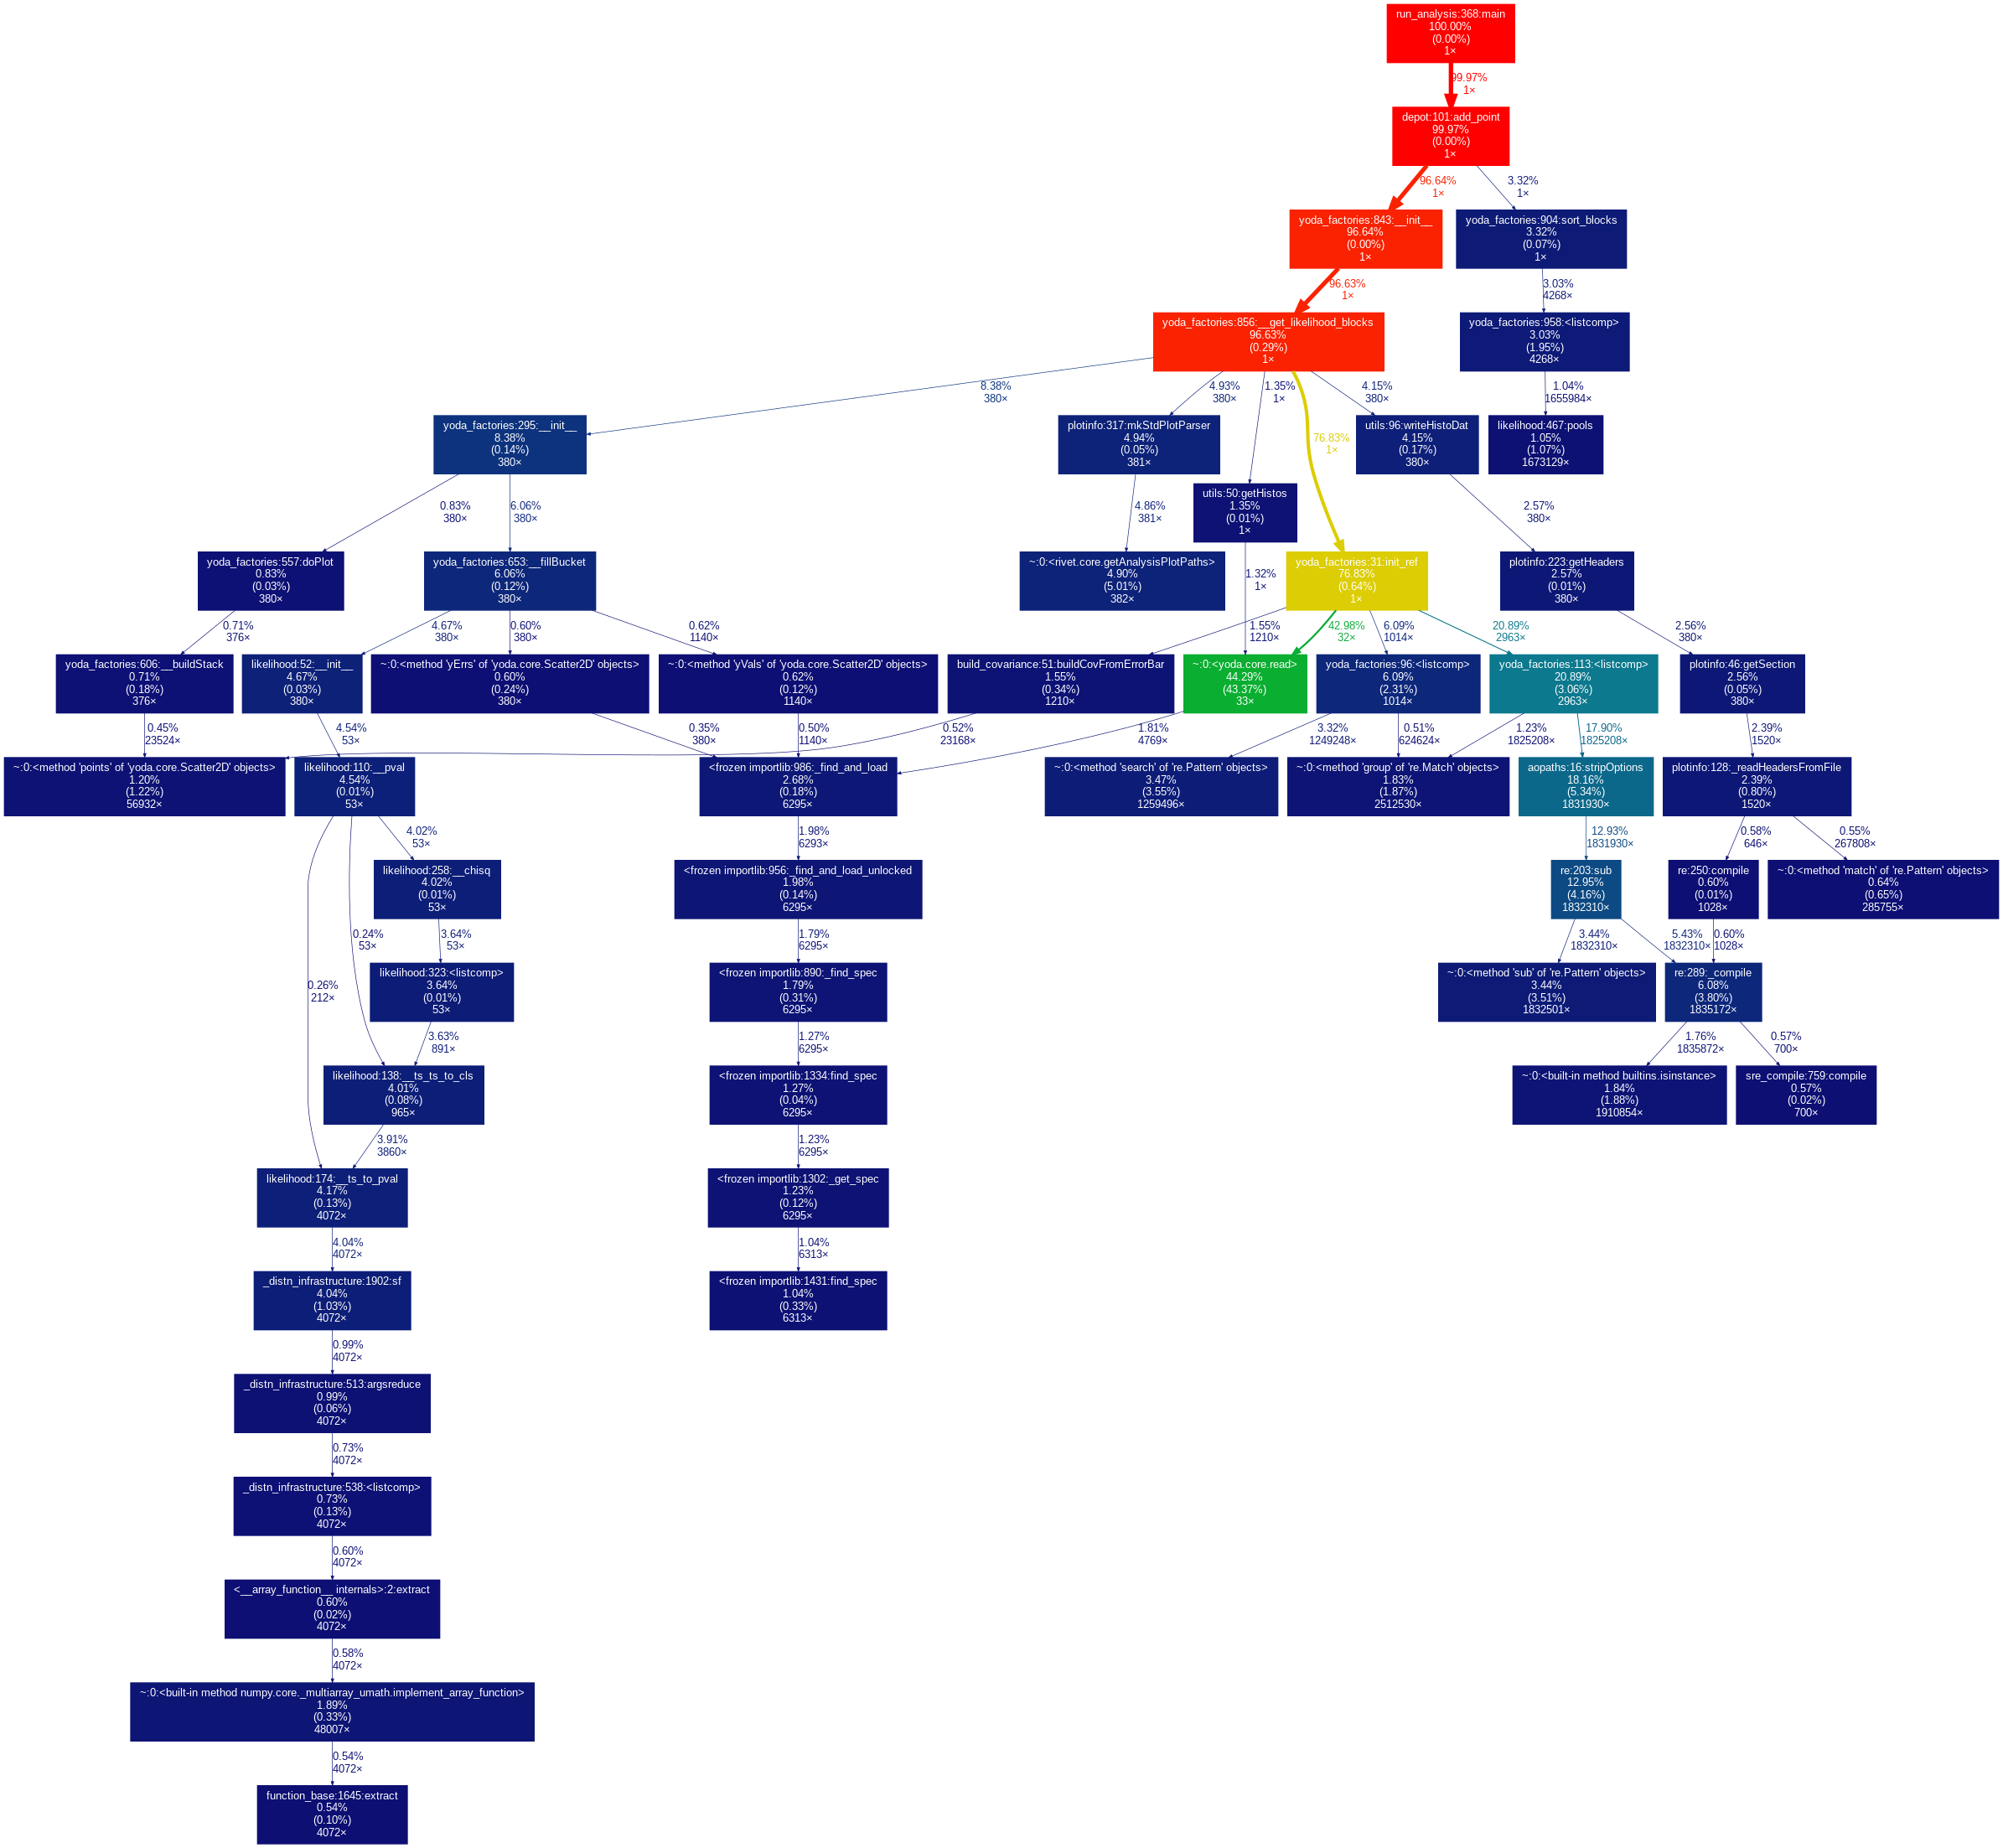
\includegraphics[scale=0.2]{plots/initial_contur_single_yoda.png}
\caption{\textbf{Contur} single \textbf{YODA} run starting point - Example \textbf{gprof2dot}}
\label{fig:single_yoda_start_profile_gprof2dot}
\end{figure}

We can see example of the dot plots produced by \textbf{gprof2dot} in figure \ref{fig:single_yoda_start_profile_gprof2dot} above. This plot is visualising the same single \textbf{YODA}  run as in figure \ref{fig:single_yoda_start_profile_snakeviz}, so is a good way of demonstrating the complementary nature of the icicle plot and the dot plots for visualising our profiling results. Following the colouring scheme in the dot plot (red to yellow to green) the observation we previously made using the icicle plot about the weight of data reading in the runtime can be seen in the dot plot where we can see c.a. $42\%$ of run time is spent reading \textbf{YODA} files.

\section{Initial Profile Results}
In the previous section while introducing the visualisation tools we gave the initial profiling results resulting from running \textbf{Contur} on a single \textbf{YODA} file (see figure \ref{fig:single_yoda_start_profile_snakeviz} and \ref{fig:single_yoda_start_profile_gprof2dot} ) before any optimisation of the code was attempted. 

As previously discussed, in practical settings \textbf{Contur} is generally run on a grid of \textbf{YODA} files as opposed to a single \textbf{YODA} file, so along with our initial single \textbf{YODA} run profile we will also perform an initial profile of \textbf{Contur} on a test grid. The grid we use to perform this profile is a $10 \times 10 $ grid, so composed of $100$ \textbf{YODA} files in total, we will use this reference grid throughout to profile \textbf{Contur's} grid run.

In figure \ref{fig:grid_yoda_start_profile} below we see the icicle plot for the grid run, from this we can see that for the grid of 100 \textbf{YODA} files we have a run time of around $1100$ seconds or close to $20$ minutes. 
\begin{figure}[H]
\centering
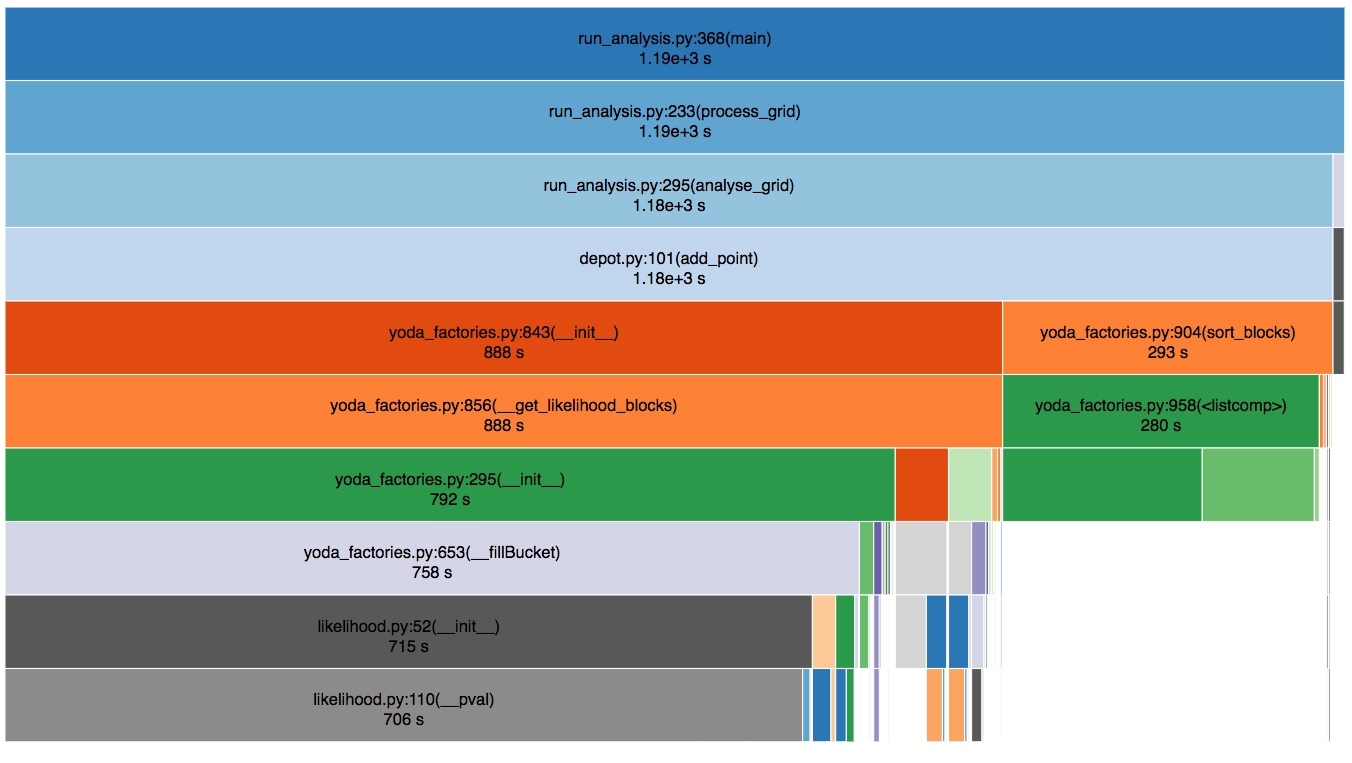
\includegraphics[scale=0.30]{plots/initial_contur_grid_profile_two.png}
\caption{\textbf{Contur} grid run - icicle plot}
\label{fig:grid_yoda_start_profile}
\end{figure}

We can also see from the plot that the main contribution to the run time seems to be coming from two blocks of the code. This is best seen in the dot plot figure \ref{fig:grid_yoda_start_profile_dot} below where we can see that the \texttt{sort\_blocks()} method contributes c.a. $25\%$ of the run and the \texttt{ts\_to\_pval()} method which contributes c.a. $49\%$, so both of these methods in combination are close to three quarters of the run time for the \textbf{Contur} grid run.

\begin{figure}[H]
\centering
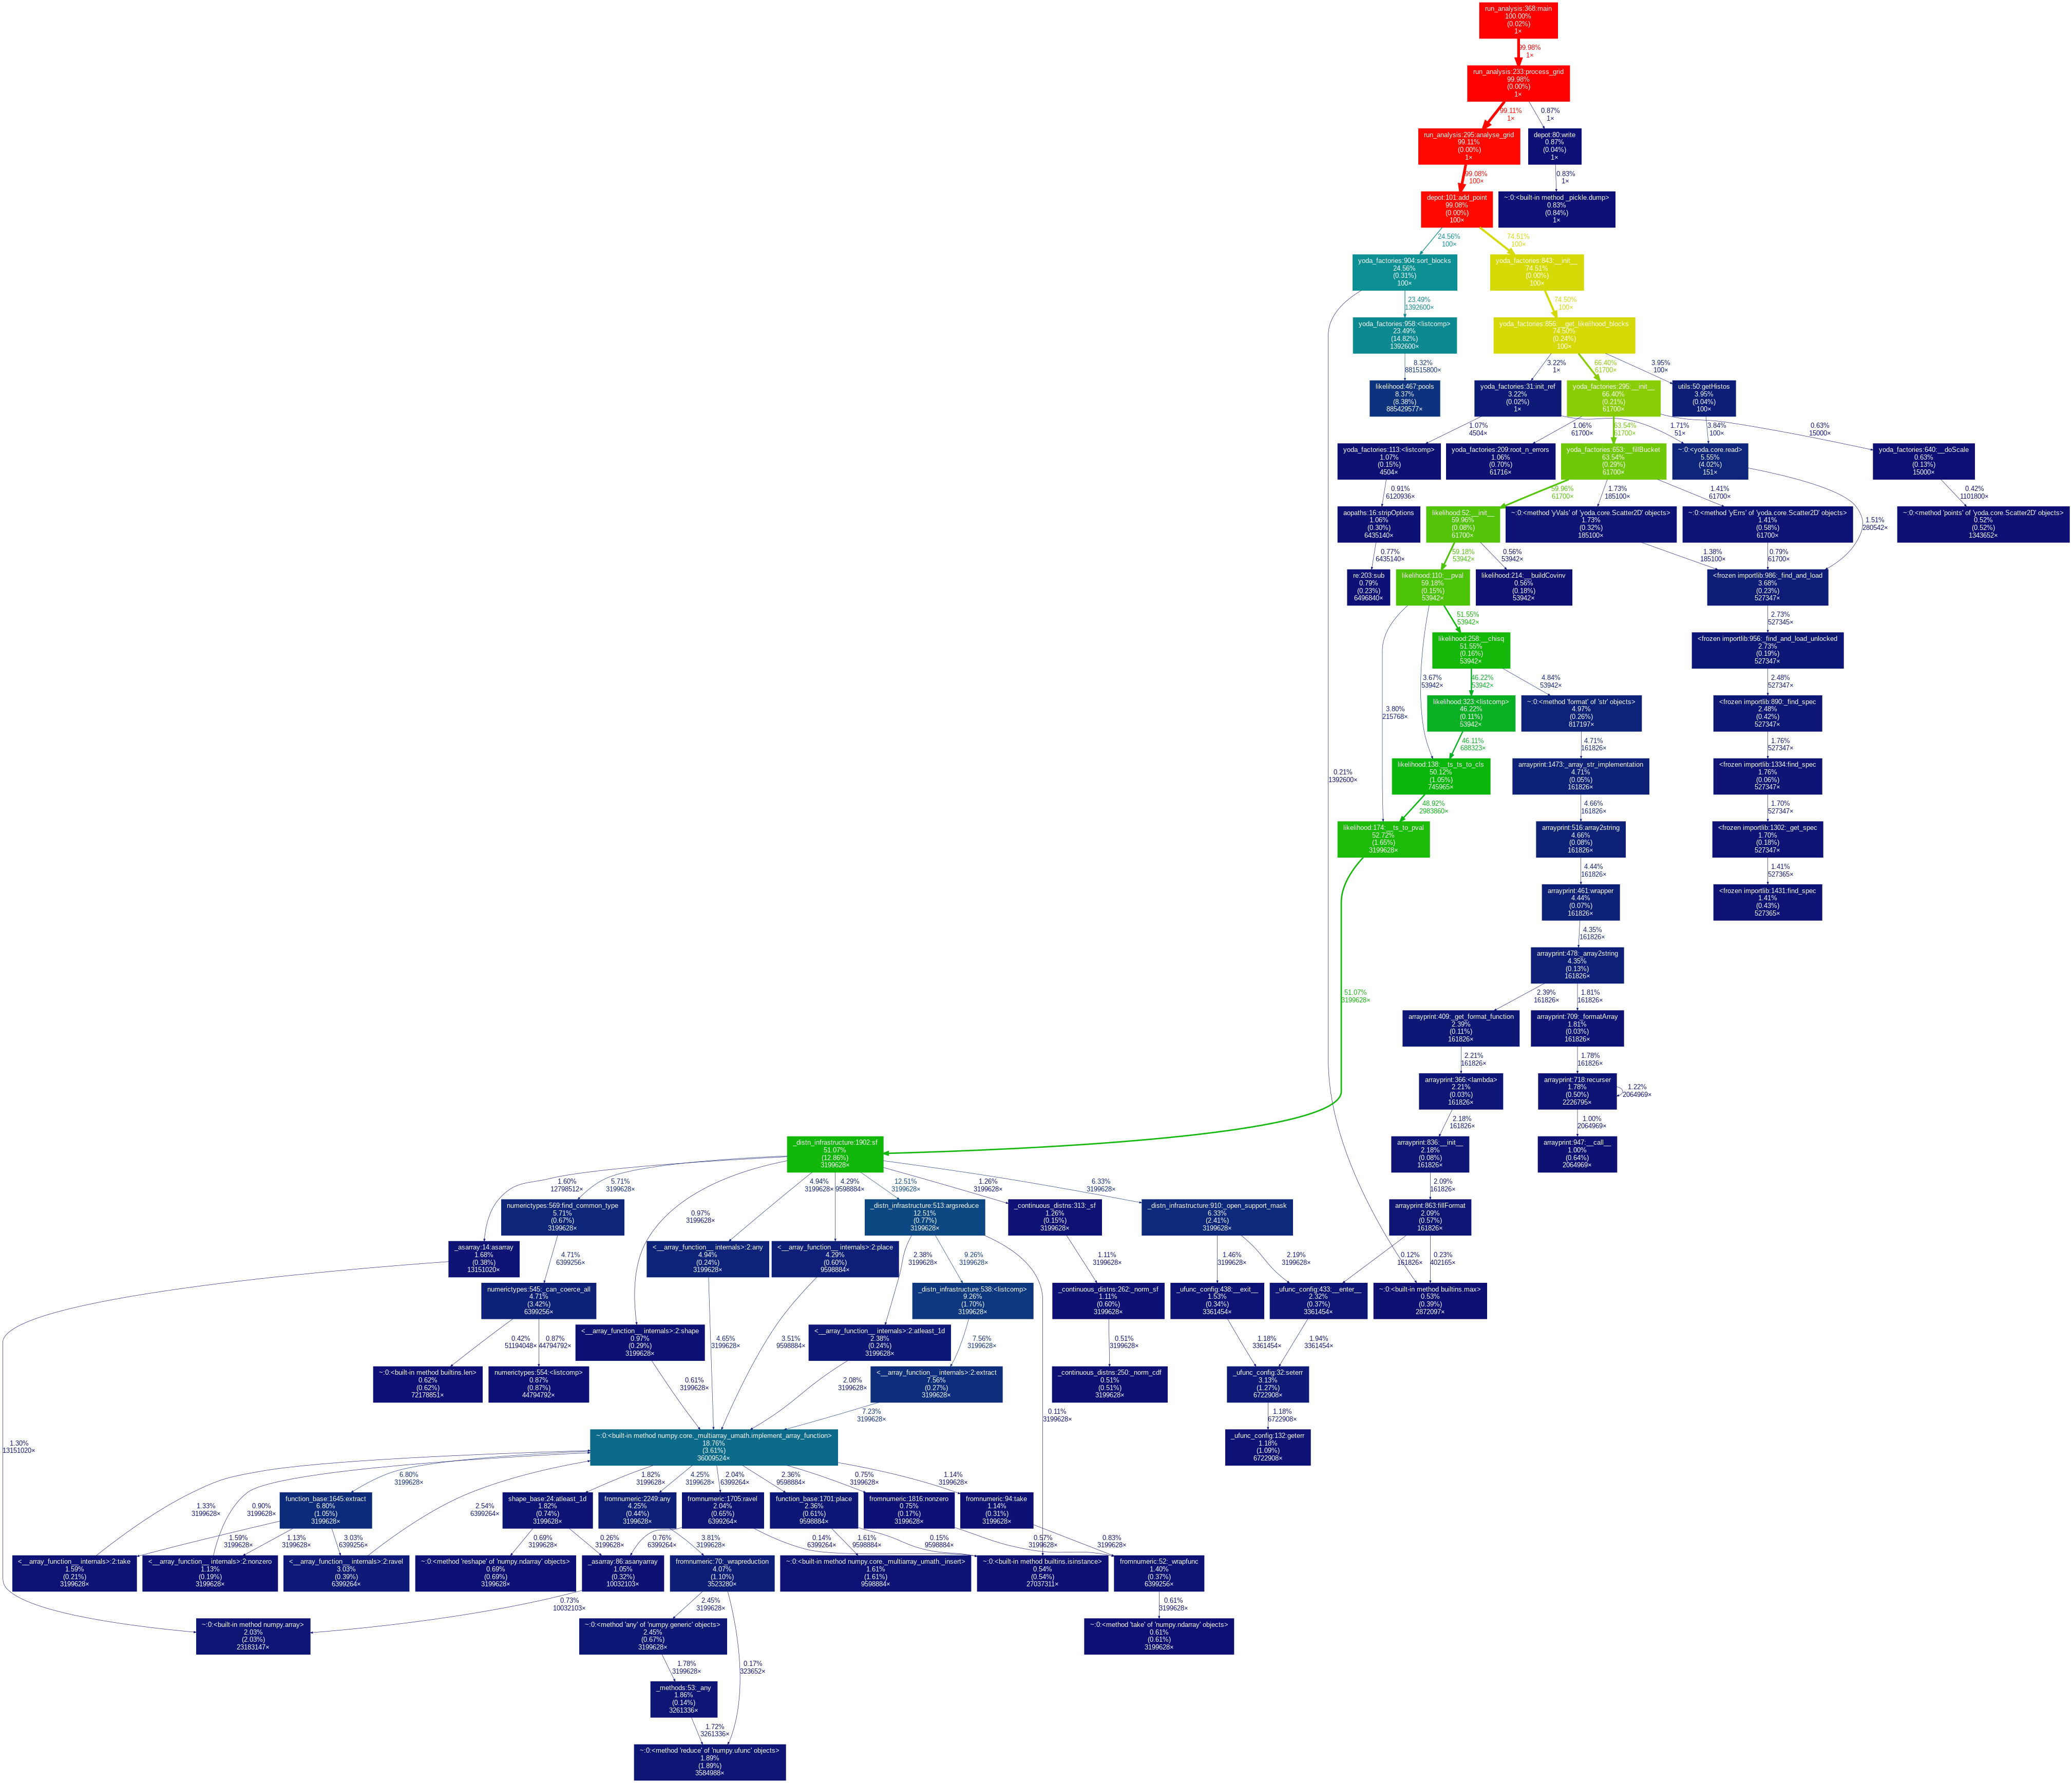
\includegraphics[scale=0.12]{plots/initial_contur_grid_two.png}
\caption{\textbf{Contur} grid run - dot plot}
\label{fig:grid_yoda_start_profile_dot}
\end{figure}





\chapter{Optimising Contur}
\label{chapterlabel4}

% This just dumps some pseudolatin in so you can see some text in place.
\blindtext

\chapter{Testing Contur}
\label{chapterlabel5}

% This just dumps some pseudolatin in so you can see some text in place.
\blindtext

\chapter{General Conclusions}
\label{chapterlabel6}

% This just dumps some pseudolatin in so you can see some text in place.
\blindtext

\phantomsection
\addcontentsline{toc}{chapter}{Appendices}

% The \appendix command resets the chapter counter, and changes the chapter numbering scheme to capital letters.
%\chapter{Appendices}
\appendix
\chapter{Viewing Profiling Results}
\label{appendixlabel1}
All profiling results shown in this thesis are saved in the Git repository located \href{https://github.com/SeanBrayUCL/contur_thesis}{here}. The repository contain a Read.Me file which should make the navigation of the profiling results clear. 

To briefly summarise, the \texttt{profiles} folder in the repository contains all the profiles, its contents are shown in figure \ref{fig:profiles_folder} below. The \texttt{starting\_point} folder is the initial profile before optimisation, it contains a \say{prof} file which can be read by \textbf{Snakeviz} to create the browser interface discuss in section \ref{chapterlabel3}, additionally the folder also contain a png file which is the dot plot produced \textbf{gprof2dot} and discussed further in section \ref{chapterlabel3}.

\begin{figure}[H]
\centering
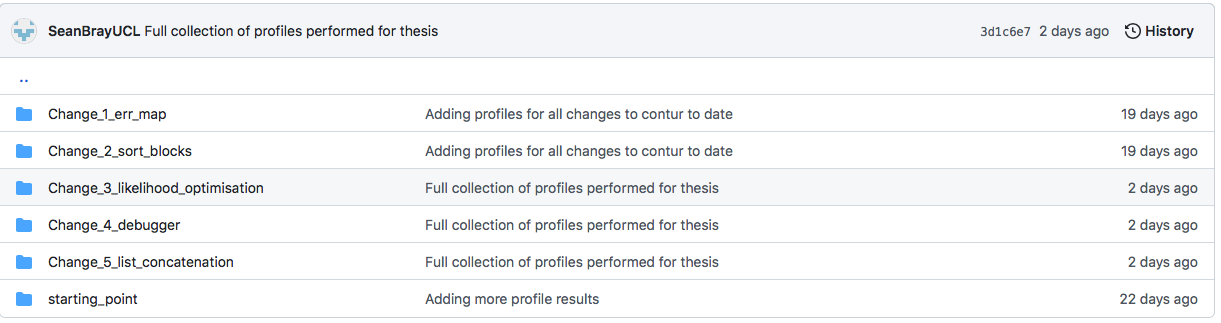
\includegraphics[scale=0.3]{plots/profiles_folder.png}
\caption{Profiles Folder}
\label{fig:profiles_folder}
\end{figure}

Each of the subsequent numbered folders are structured the same as the \texttt{starting\_point} folder. They each contain an updated profile of \textbf{Contur} after an optimisation change has been made. The optimisation changes accumulate across the folders, so the profile in folder \texttt{Change\_5\_list\_concatenation} contains all the optimisation changes, so can be taken as the complete post optimisation \textbf{Contur} profile.

\chapter{Viewing Code Written For Project}
All code written for this project, with one exception, can be found in the main \textbf{Contur} repository\cite{contur_main}. Links to specific commits made by this author can be found throughout this thesis, the approach taken has been to include a footnote with a link to the specific commits when discussing code changes in the thesis. A quick overview of code contributions to the main repository by this author can also be seen via the contributors page of the main \textbf{Contur} repository\cite{contur_main}.

 
% You could separate these out into different files if you have
%  particularly large appendices.

\begin{thebibliography}{9}
\bibitem{ufo} 
UFO - The Universal FeynRules Output,
\\\texttt{https://arxiv.org/abs/1108.2040}

\bibitem{herwig} 
Herwig - Event Generator,
\\\texttt{https://herwig.hepforge.org}

\bibitem{yoda} 
Yoda,
\\\texttt{https://yoda.hepforge.org}

\bibitem{contur_manuel} 
Contur User Manuel,
\\\texttt{https://arxiv.org/abs/2102.04377}

\bibitem{cProfile} 
cProfile Documentation,
\\\texttt{https://docs.python.org/3/library/profile.html}

\bibitem{contur_main} 
Main repository with Contur code,
\\\texttt{https://gitlab.com/hepcedar/contur}

\bibitem{snakeviz} 
Snakeviz Package,
\\\texttt{https://jiffyclub.github.io/snakeviz/}

\bibitem{gprof2dot} 
gprof2dot Package,
\\\texttt{https://github.com/jrfonseca/gprof2dot}

\bibitem{pytest} 
Python pytest Documentation,
\\\texttt{https://docs.pytest.org/en/6.2.x/}

\bibitem{HEPData} 
HEPData Repository,
\\\texttt{https://arxiv.org/abs/1704.05473}

\bibitem{Rivet} 
Rivet Library,
\\\texttt{https://rivet.hepforge.org}

\bibitem{cls} 
CLS Technique,
\\\texttt{https://doi.org/10.1088/0954-3899/28/10/313}



\end{thebibliography}


% All done. \o/
\end{document}
